\chapter{How does Wifi work}
Access point is a device where we can connect to 
the WLAN network (e.g a router).

When this device is up it starts by choosing a channel
of the bandwidth to use, once this is finished it starts 
transmitting beacons each $T_{beacons}ms$ (usually $100ms$)
Each beacon contains information about the AP, such as the 
BSSID (name of the network), supported transmission rates,
and other charactersitics\dots

Then we have stations (STA), devices that we use to connect
to AP, e.g. computers, phones, etc

\begin{figure}[htbp]
    \centering
    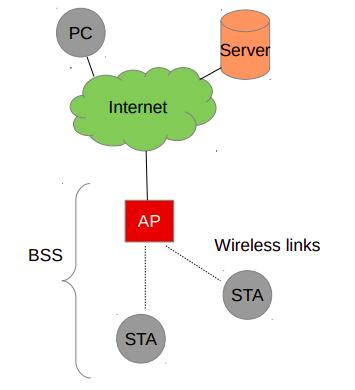
\includegraphics[width=0.6\textwidth]{infrastructure.png}
    \label{infrastructure}
\end{figure}
\section{Link layer}
The typical connection we'll see is formed by multiple nodes,
is half-duplex (the connection allows communication in both
directions but only one direction at a time).
The channel access arbitration is done using the 
\textbf{Distributed Coordination Function (DCF)} which consists
of:
\begin{itemize}
    \item CSMA protocol
    \item Backoff (BEB)
    \item Stop \& Wait ARQ protocol, for packet retransmissions
\end{itemize}
\subsection{DCF}
\subsection{Automatic ReQuest protocol (Stop \& Wait)}
Where unconfirmed packages are retransmitted until they are 
acknowledged or discarded. There is a maximum number of retransmissions $R_{\max}$
Between packages we have the \textbf{Short Interframe Space (SIFS)}
\begin{figure}[htbp]
    \centering
    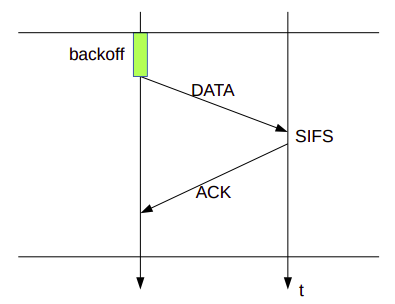
\includegraphics[width=0.7\textwidth]{arq.png}
    \caption{ARQ}
    \label{ARQ}
\end{figure}